\documentclass{article} % This command is used to set the type of document you are working on such as an article, book, or presenation

\usepackage{geometry} % This package allows the editing of the page layout
\usepackage{amsmath}  % This package allows the use of a large range of mathematical formula, commands, and symbols
\usepackage{graphicx}  % This package allows the importing of images
\graphicspath{ {./images/} }

\usepackage{comment}


\newcommand{\maketitletwo}[2][]{\begin{center}
        \Large{\textbf{Course Notes for Financial Markets} \\
            			   Yale University} % Name of course here
        \vspace{5pt}
        
        \normalsize{Daniel Girvitz  % Your name here
        
        \today}        % Change to due date if preferred
        \vspace{15pt}
        
\end{center}}

\begin{document}
     \maketitletwo[]
     
     \section*{Week 1}
     
     	\subsection*{Lesson 1}
     	- "Financial institutions are a pillar of civilized society, directing resources across space and time to their best uses, supporting and incentivizing people in their productive ventures, and managing the economic risks they take on. The workings of these institutions are important to comprehend if we are to predict their actions today and their evolution in the coming information age."
     	\\
     	\\
     	- as individuals, we can do little, thus, there is a point in joining an organization of our fellows, through which we can accomplish more -- this is a fundamental principle of human life
     	\\
     	\\
     	- massage therapists are more likely to find jobs than all of economists, astronomers, sociologists, political scientists, and mathematicians combined... LOL!
     	\\
     	\\
     	- finance is a technology, for good or evil
     	\\
     	\\
     	- 
     	
     	\subsection*{Lesson 2}
     	
     		\subsubsection*{VAR and VaR}
     	
     		- VAR -- variance ie a measure of variability \\
     		\\
     		- VaR -- value at risk \\
     		\\
     		- 'VaR' was invented after the stock market crash of 1987 \\
     		\\
     		- VaR is usually quoted in units of \$ for a given probability and time horizon \\
     		\\
     		- 1\% one-year VaR of \$10 million means: 1\% chance that a portfolio will lose \$10 million in a year \\
     		
     		\subsubsection*{Stress Test}
     		
     		- It's not a basic statistical concept, it's a measure \\
     		\\
     		- It's a method of assessing risks to firms or portfolios \\
     		\\
     		- The idea of a stress test is that, let's look at a portfolio not just by its historical returns and how variable they are, but let's look at the details of the portfolio and ask what vulnerabilities there are for various kinds of financial crisis because what actually stresses firms the most are crisis \\
     		\\
     		- The stress test is a test usually ordered by government to see how some firm will stand up to a financial crisis. \\
     		\\
     		- The Dodd-Frank Act in the United States of 2010 requires the Federal Reserve to do annual stress tests for non-bank financial institutions it supervises. \\
     		\\
     		-The Dodd-Frank Wall Street Reform and Consumer Protection Act was passed into Federal law on July 21, 2010 as a response to the financial crisis of 2007 to 2008. This Act constitutes the most significant changes to U.S. financial regulation since the regulatory reform that followed the Great Depression \\
     		\\
     		- The United Kingdom, China and other countries (++ EU) all do stress tests now but the question is, do they work? Well, there is a growing amount of skepticism that they can really measure what will happen in the next crisis. Anat Admati is a professor at Stanford who's been arguing it's all garbage. You can't. These guys who are trying to predict what will happen to these companies in a financial crisis, they just don't have the imagination and understanding of how things work out in a panic, in a financial panic and she thinks that they are just way underestimated. \\
     		\\
     		- there is a push for whitewashed Stress Tests... because a bad one wil generate bad publicity -- ie ethical problem \\
     		
     		\subsubsection*{S\&P 500}
     		
			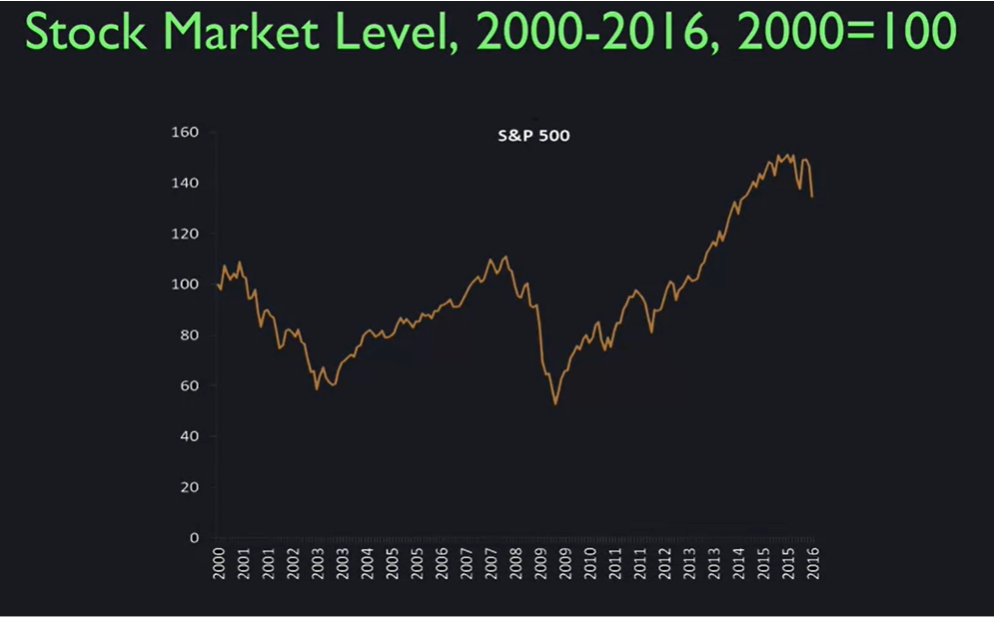
\includegraphics[width=\textwidth]{S&P 500 -- 2000-2016.png} \\
			\\
     		- It's an average of 500 stocks. So if they were all independent of each other, the Law of Large Numbers would make the stock market as a whole almost constant. But, in fact, it's actually gone up hugely. So there's definite dependence across stocks \\
     		\\
     		- used as a benchmark for returns \\
     		\\
     		- making assumption that it's hard to forecast ... nobody knows the future!!!\\
     		\\
     		- we're going to look at risk as something that we can quantify by looking at the standard deviation of past risks and not focus on what's new right now \\
     		\\
     		- every company has its own culture and it produces a strange outlier effect \\
     		\subsubsection*{Market risk vs. idiosyncratic risk}
     		- market risk: a company's risk in reaction to the stock market \\
     		\\
     		- idiosyncratic risk: a company's risk ... ie what if something happens to the company \\
     		\\
     		 \subsubsection*{Joe McNay}
     		 - \\
     		 \\
     		 \subsubsection*{Distribution and Outliers}
     		 - Cauchy Distribution ... sounds useful. \\
     		 \\
     		 - generally data is normally-distributed, but crazy events happen occasionally (a fat tail distribution) \\
     		 \\
     		 -  \\
		\\
		\subsubsection*{Chalk Talk - Covariance}
		- \\
		\\
		\subsubsection*{} 

	\subsection*{Lesson 3}

		\subsubsection*{Insurance}
		- policy-holders have a contract with a company to protect against some well-defined risk, for which they pay a premium (regular payment) to the insurance company
		
		\subsubsection*{Fundamental Insurance Principles and Issues}
		- \textbf{Risk Pooling} is the source of all value in insurance (a risk to one person is not a risk to society) \\
		\\
		- If \textit{n} policies, each has independent probability p of a claim, then the number of claims follows the binomial distribution. The sd of the fraction of policies that result in a claim is $\sqrt{p(1-p)/n}$ \\
		\\
		- Law of Large Numbers, as n gets large sd approaches 0 \\
		\\
		- LLN important as it guarantees stable, long-term results
		 \\
		- moral hazard - people insured take more risks \\
		\\
		- selection bias 
		
		\subsubsection*{Insurance Milestones}
		- goes back to Ancient Rome \\
		\\
		- rapid development of actuarial theory starting in 1600s with notion of probability 
		\\
		- Morris Robinson Mutual Life of NY 1840 \\
		\\
		- Henry Hyde Equitable Life Assurance Society 1880s: large cash value (psychological framing) \\
		\\
		- Viviana Zelizer \\
		\\
		- life insurance is to protect the death of a father or mother while young \\
		\\
		\subsubsection*{Insurance is a Local Phenomenon}
		
		\subsubsection*{Dodd Frank Act in the US}
		- created a federal insurance office \\
		\\
		- monitors insurance companies, looking for systemic risk \\
		\\
		\subsubsection*{State Insurance Guarantee Funds}
		- most US states have guarantee funds protecting insurance against failure of the insurance company \\
		\\
		- The first state to set up such a fund was New York, in 1941 \\
		\\
		- Protects individuals, not businesses or group insurance \\
		\\
		\subsubsection*{Disasters}
		- 
		
	\subsection*{Lesson 4}
		- diversification is an alternative to insurance \\
		\\
		- risk is inherent to investing! \\
		\\
		- without risk, there could be no returns \\
		\\
		- manage risks with diversification \\
		\\
		- if you can quantify risks and returns, why should it be different from one person to another ... ie most ppl converge on the market portfolio \\
		\\
		- Capital Asset Pricing Model (CAPM) ... how to optimize risk... read about Harry Markowitz!!! \\
		\\
		- Hedge funds are investment companies not approved for the general, retail market, so they're not allowed to advertize, and are consequently not well-known \\
		\\
		- only accredited investors are allowed to invest in hedge funds \\
		\\	
		- banks \& other financial institutions are very interconnected \\
		\\
		- \textit{The Black Swan} by Nassim Taleb \\
		\\
			\subsubsection*{CAPM, Optimal \& Efficient Portfolios}
			- Mutual Fund Theorem??? \\
			\\
			- beta \\
			\\
			- idiosyncratic risk averages out \\
			\\
			- only market risk matters \\
			\\
			- negative beta stocks help in a better way: help offset market shocks, help reduce variance of returns\\
			\\
			- credit default swaps??? \\
			\\
			- 
			\subsubsection*{Gordon Growth Model}
			- infinite sum which is pretty cool!!! \\
			\\
		
     \section*{Week 2}
     
     	\subsection*{Lesson 5}	
     	- invention takes a long time \\
     	\\
     	- no wheeled suitcases until 1972 ... lol \\
     	\\
     	- financial innovation: repurpose risk so that it's appealing\\
     	\\
     	\subsubsection*{Limited Liability}
     	- birth in New York in 1811: A law was passed: Investors in stocks can never be pursued for mistakes of the company invested in \\
     	\\
     	- discovered investor psychology favours limited liability \\
     	\\
     	\subsubsection*{Inflation Indexed Debt}
     	- history shows many examples of nominal debt being wiped out in real terms by high inflation \\
     	- 4\% a year inflation - you lose half your money in 20years \\
     	\\ 
     	- In economics, money is often defined in terms of the three functions it provides: a store of value, a unit of account and a medium of transaction.
     	\subsection*{Lesson 6}	
     	
     		\subsubsection*{Forecasting \& Random Walk}
     		- Random walks such that changes are independent of past changes and so are completely unforecastable \\
     		\\
     		- \textit{A Random Walk Down Wall Street} - lol author contradicts himself and doesn't completely believe in the Random Walk Process\\
     		\\
     		- Is the Stock Market a Random Walk or an AR(1)???
     		\subsubsection*{Efficient Market Hypothesis}
     		- read up about it! \\
     		\\
     		- in short: \\
			\\
			- stock market has a tendency to fall before a recession \\
			\\
			-     		
    
     \section*{Week 3}
     
     	\subsection*{Lesson 8}
     	
     		\subsubsection*{1982 Savings Acct.}
     		
     		- The "term" is the minimum amount of time that must pass before you can withdraw your money without penalty \\
     		\\
     		- 
     		
     		\subsubsection*{Federal Funds and Interest Rates}
     		
     		- \textit{Capital and Interest} Eugen von Bohm-Bawerk \\
     		\\
     		- \textit{Theory of Interest} by Irving Fisher \\
     		\\   	
     		
			\subsubsection*{Compound Interest}
			
			- compounded $n$ times per year: $ (1+r/n)^{nt} $ \\
			\\
			- continuous compounding: $e^{rt}$
     		
			\subsubsection*{Discount Bonds}     		
     		-  no coupons ... why buy it? Really cheap \\
     		\\
     		- 
     		\subsubsection*{Inflation and Interest Rates}
     		- John Bates Clark ... Real interest rates
     		
     		\subsubsection*{Leverage}
     		- leveraging means you're putting more money into an asset than you have (ie borrowed money) \\
     		\\
     		- 
     		
		\subsection*{Lesson 8}     
		
		- whoops... forgot to save...	
		
		\subsection*{Lesson 9}
		
		- whoops... forgot to save...   
     		
			\subsubsection*{Dilution}
     			- if the company gives away new shares, current shares become worth less... \\
     			- 	
        		  \\
     		-   	
     		\subsubsection*{Share Repurchase}
     			- value of the firm goes down by the amount they spent on shares outstanding \\
     			- 	
        		  \\
     		- 
     		
     		\subsubsection*{Price as PDV of Expected Dividends}
     			- value of the firm goes down by the amount they spent on shares outstanding \\
     			- 	
        		  \\
     		-     
 
     \section*{Week 4}
     
     	\subsection*{Lesson 10}
     	
     		\subsubsection*{Recessions}
     		- historically, inverted yield curves tend to be followed by recessions \\
     		\\
     		- 
     	
			\subsubsection*{History of Mortgage Lending}
     		- historically, goes back to Tang Dynasty in China \\ \\
     		-      	
     	
     		\subsubsection*{Commercial Real Estate Vehicles}
     		- in the US, only for accredited investors \\ \\ 
     		-  Real Estate Investment Trusts (REITS) \\ \\
     		
     		\subsubsection*{Mortgages}
     		- really has its own history \\ \\
     		- Federal Housing Administration (FHA) by Roosevelt in 1934 \\ \\
     		- lots of mortgage types
     		
     		\paragraph*{Question:}
     		Which of the following is a reason that the 30 year mortgage rate is higher than the 10 year treasury bond YTM? \\ \\


FALSE: Mortgages usually are adjusted to account for inflation. \\ \\


FALSE: Housing prices have historically been more stable than treasury bonds. \\ \\


FALSE: A treasury bond is riskier than a mortgage. \\ \\


TRUE: There are overhead costs to managing a mortgage. \\ \\
     	
     		\subsubsection*{PMI, CMOs, CDOs}
     		- really has its own history \\ \\
     		- Federal Housing Administration (FHA) by Roosevelt in 1934 \\ \\
     		- lots of mortgage types \\ \\
     		- Collateralized Mortgage Obligation (CMO) ... pools of mortgages sold to investors \\ \\
     		
     		\subsubsection*{A Fix Begun in Europe}
     		- liar's loan: a mortgage issued to a person who did not show evidence of a job and/or good record \\ \\ 
     		- 
     		
     		\subsubsection*{Excess Reserves}
     		- govts decreed banks need to keep a certain amount of cash on reserve to meet any sudden increase in demand from their depositors \\ \\
     		- excesses reserves are reserves banks hold beyond what they're required to hold by regulation \\ \\ 
     		- adverse selection ??? \\ \\
     		- author: Edward Miller ... article about short selling \\ \\ 
     		- 
     		
     	\subsection*{Lesson 11}
     	
     		\subsubsection*{Regulation and Human Behavior}
     		- microprudential: \\ \\
     		- macroprudential: regulation to prevent big bad-events \\ \\
     		
     		\subsubsection*{Board of Directors}
     		- must be loyal to shareholders \\ \\ 
     		- ought to prevent tunneling (stealing money and/or valur from a company) \\ \\ 
     		
			\subsubsection*{Trade Groups}
			- first stock exchange in the US (not in the world) founded in 1792	\\ \\
			- 
			
			\subsubsection*{Local Regulation}
			- 1934 - birth of SEC \\ \\
			- \textit{Other Peoples' Money} by Louis Brandeis \\ \\
			- 
	
			\subsubsection*{National Regulation}
			- corruption decreases as countries develop \\ \\ 
			- \textit{Democracy and Finance} by William O. Douglas \\ \\
			- 
			
			
			
				     		
\end{document}